\beginsong{On my honour}[wuw={Cindy Dasch, kanadisches Pfadfinderlied, 1993}, pfii={192}, pfiii={4}]

\markboth{\songtitle}{\songtitle}

\centering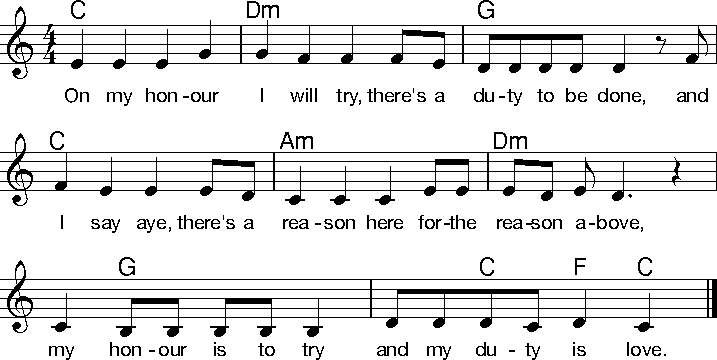
\includegraphics[width=1\textwidth]{Noten/Lied074.pdf}	

\beginverse
\[C]People don't need to \[Dm]know my name.
If I \[G]hurt someone, then \[C]I'm to blame.
If I \[Am]helped someone, then \[Dm]I helped me,
and \[G]that's the way, that \[C]it \[F]should \[C]be.
\endverse

\beginverse
^I'be tucked away a ^song or two;
If you're ^feeling low, there's ^one for you,
If you ^need a friend, then ^I will come,
There are ^many more, where ^I ^come ^from.
\endverse

\beginverse
^Come with me where the ^fire burns bright,
You can ^even see better in a ^candle's light,
You can ^find more meanings in a ^campfire's glow,
then ^you'll ever get in a ^year ^or ^so.
\endverse

\beginverse
^We've made a promise do ^always keep,
We'll sing '^Day Is Done', be^fore we sleep,
We'll be ^scouts together and ^when we're gone,
they'll ^still be a-trying and a-^singing ^this ^song.
\endverse

\endsong

\beginscripture{}

\endscripture

\begin{intersong}	

\ifthenelse{\boolean{pics}}{
\ThisLRCornerWallPaper{1}{Bilder/onmyhonour.png}
}{}


\end{intersong}